\section{Uso de internet}

O uso da internet tem crescido exponencialmente desde o ano 2000. Conforme a figura \ref{fig:individuals_using_internet_itu}, iniciando em menos de 2\% em 2000, o uso da internet atingiu um índice de mais de 60\% em 2024 globalmente. 

\begin{figure}[ht]
    \centering
    \caption{Uso pessoal de internet pelo mundo (2000-2024)}
    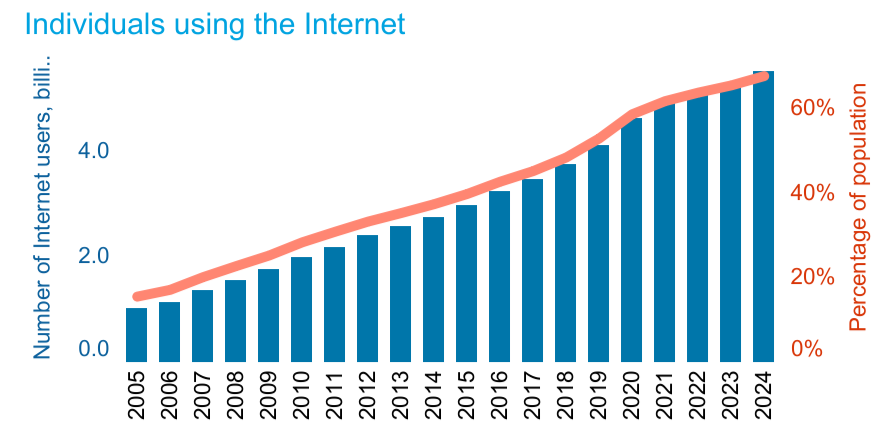
\includegraphics[width=0.78\linewidth]{figuras/internet/individuos_uso_internet_itu.png.png}
    \label{fig:individuals_using_internet_itu}
    \\ \footnotesize{Fonte: \cite{ITU_uso_internet_mundo}.}
\end{figure}

O crescimento do uso da internet no Brasil foi tão exponencial quanto a tendência do crescimento global. O notório crescimento no Brasil está representado na figura \ref{fig:crescimento_internet_brasil_itu}.

\begin{figure}[ht]
    \centering
    \caption{Crescimento do uso de internet no Brasil (2000-2023)}
    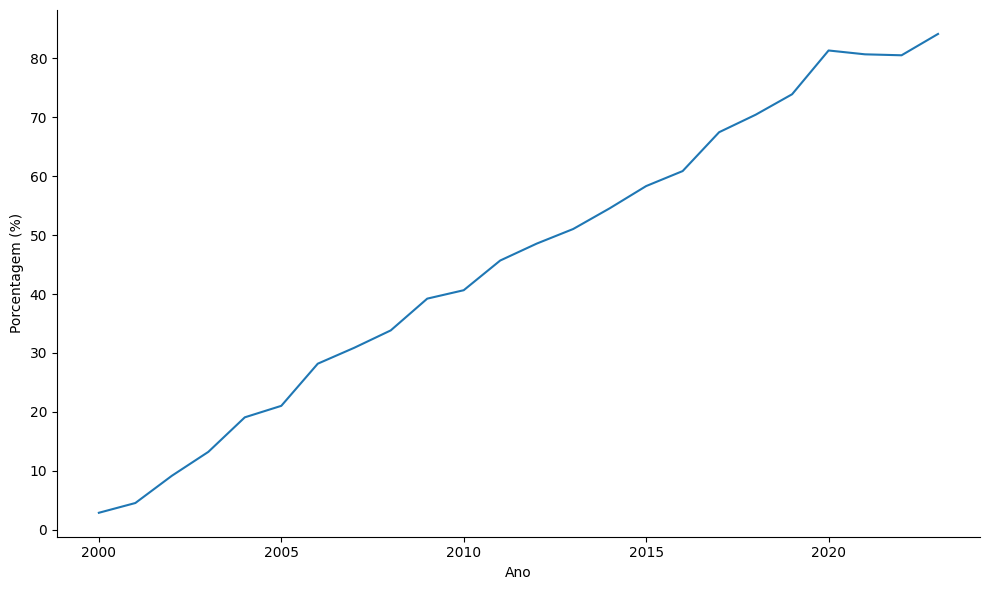
\includegraphics[width=1\linewidth]{figuras/internet/lineplot_uso_internet_brasil_itu.png}
    \label{fig:crescimento_internet_brasil_itu}
    \footnotesize{Fonte: \cite{ITU_crescimento_uso_internet_brasil}.}
\end{figure}

A linha de tendência do crescimento demonstra que em 2000 o uso de internet no Brasil era um pouco mais do que 0\%; em 2020, a porcentagem ultrapassou os 80\%. A figura \ref{fig:uso_internet_brasil_itu} mostra as porcentagens por ano desde 2000 até 2023. Embora houvesse dois retrocessos em 2021 e 2022, fazendo o índice atingir os 80\%, ele ultrapassou a faixa dos 81\%.

\begin{figure}[ht]
    \centering
    \caption{Uso de internet no Brasil (2000-2023)}
    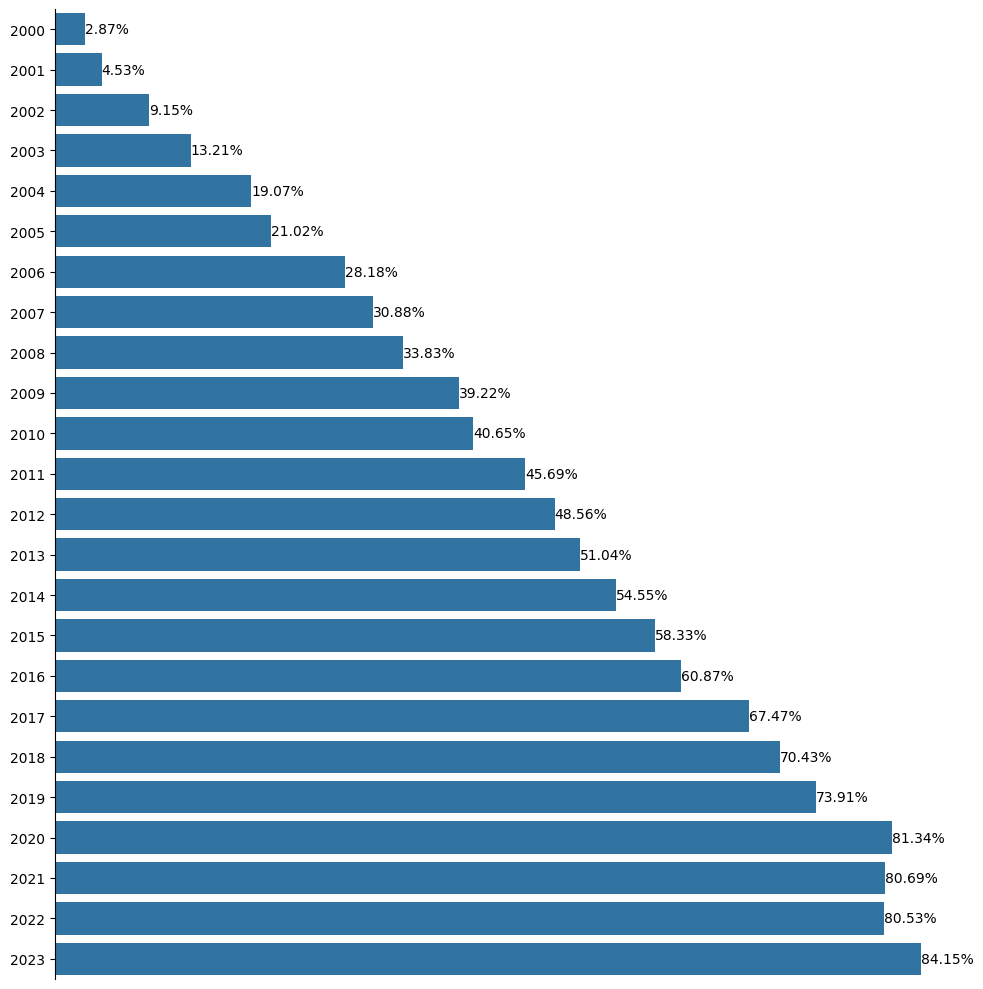
\includegraphics[width=1\linewidth]{figuras/internet/barplot_uso_internet_brasil_itu.png}
    \label{fig:uso_internet_brasil_itu}
    \footnotesize{Fonte: \cite{ITU_uso_internet_brasil}.}
\end{figure}

Visando entender melhor o crescimento do uso de internet no Brasil, fez-se uma análise em que se comparava o índice do uso de internet no Brasil, a população total do Brasil e a extensão territorial do país de 2000 até 2023 têm um coeficiente de correlação de Pearson positivo e forte. A figura \ref{fig:internet_correlacao} demonstra o resultado da análise.

\begin{figure}[ht]
    \centering
    \caption{Coeficiente de correlação de Pearson: índice do uso de internet, população total e extensão territorial}
    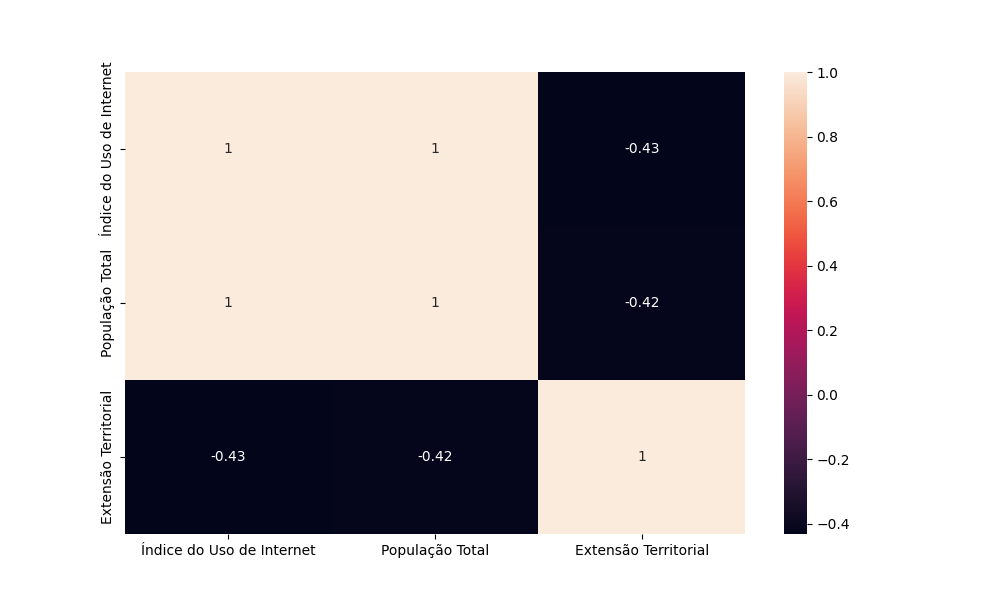
\includegraphics[width=1\linewidth]{figuras/internet/correlacao.png}
    \label{fig:internet_correlacao}
    \footnotesize{Fonte: elaboração própria.}
\end{figure}

\newpage
O coeficiente de correlação de Pearson mais positivo e forte foi entre \texttt{Índice do Uso de internet} e \texttt{População total}. De maneira contrária, \texttt{Extensão territorial} tem um coeficiente negativo com \texttt{Índice do Uso de internet} e \texttt{População total}. 

Portanto, será considerada apenas a relação \texttt{Índice do Uso de internet} e \texttt{População total}, pois o crescimento da população (até 2023) está altamente correlacionado com o crescimento do uso de internet no Brasil.

Conforme exposto pela figura \ref{fig:internet_correlacao}, o crescimento populacional (até 2023) tem forte correlação com o uso de  internet no Brasil. Assim, percebe-se tal correlação ao analisar o gráfico de crescimento projetado pela ONU, presente na figura \ref{fig:populacao_brasil}.

\begin{figure}[ht]
    \centering
    \caption{População projetada do Brasil pela IBGE (2000-2070)}
    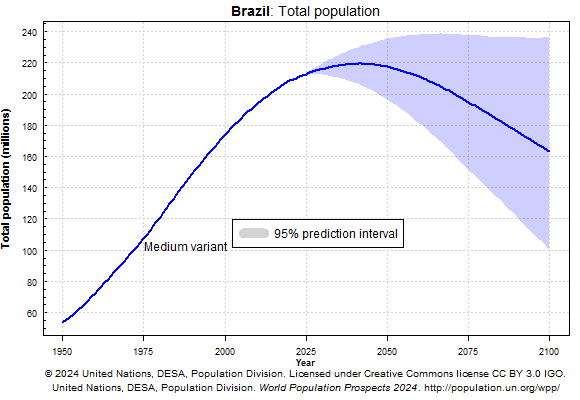
\includegraphics[width=1\linewidth]{figuras/populacao/populacao_brasil.png}
    \label{fig:populacao_brasil}
    \footnotesize{Fonte: \cite{IBGE_populacao_brasil}.}
\end{figure}

\newpage
Acrescenta-se que é importante analisar o contexto de crescimento populacional em que o coeficiente de correlação entre \texttt{Índice do Uso de internet} e \texttt{População total} da \ref{fig:internet_correlacao} está inserido. 

Percebe-se que até 2048, a população brasileira crescerá, e depois desse ano, começará a reduzir. Assim, até 2023, último ano em que o uso de internet no Brasil foi registrado pelo ITU, a correlação é alta entre uso de internet e a população total.

Como o período de mudança demofráfica ainda não se concretizou, haverá o funilamento do contexto internacional para o brasileiro. Como consequência, foram escolhidos os dados de pesquisa da PNAD Contínua Anual 2016-2019, 2021-2023. Os dados da PNAD serão extraídos da tabela 6794 (\href{https://sidra.ibge.gov.br/tabela/6794}{Pessoas de 10 anos ou mais de idade, por sexo e grupo de idade}). Nas análises, sexo e as faixa etárias de 10-13 anos e 14-17 anos não serão levadas em consideração.

A representação da realidade nacional será dividida nas 5 regiões presentes na figura \ref{fig:regioes_brasil}. \cite{HAMAM_2017} argumenta que, dividindo um país em regiões, torna-se possível compreender suas diferenças, de modo a conhecê-lo.

\begin{figure}[ht]
    \centering
    \caption{Regiões do Brasil}
    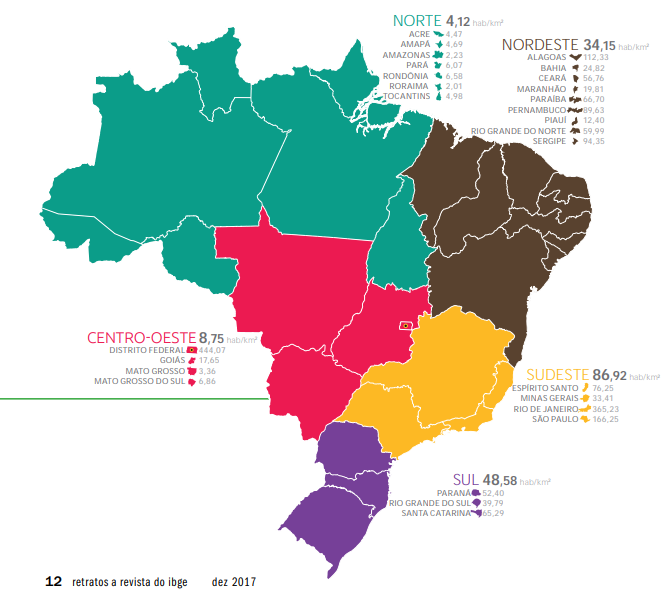
\includegraphics[width=1\linewidth]{figuras/regioes/regioes_brasil.PNG}
    \label{fig:regioes_brasil}
    \footnotesize{Fonte: \cite{HAMAM_2017}.}
\end{figure}

\newpage
Inspirando-se no argumento de \cite{HAMAM_2017}, criou-se o gráfico de distribuicao presente na figura \ref{fig:distribuicao_uso_internet_regioes}.

\begin{figure}[ht]
    \centering
    \caption{Distribuição do uso de internet pelas regioes}
    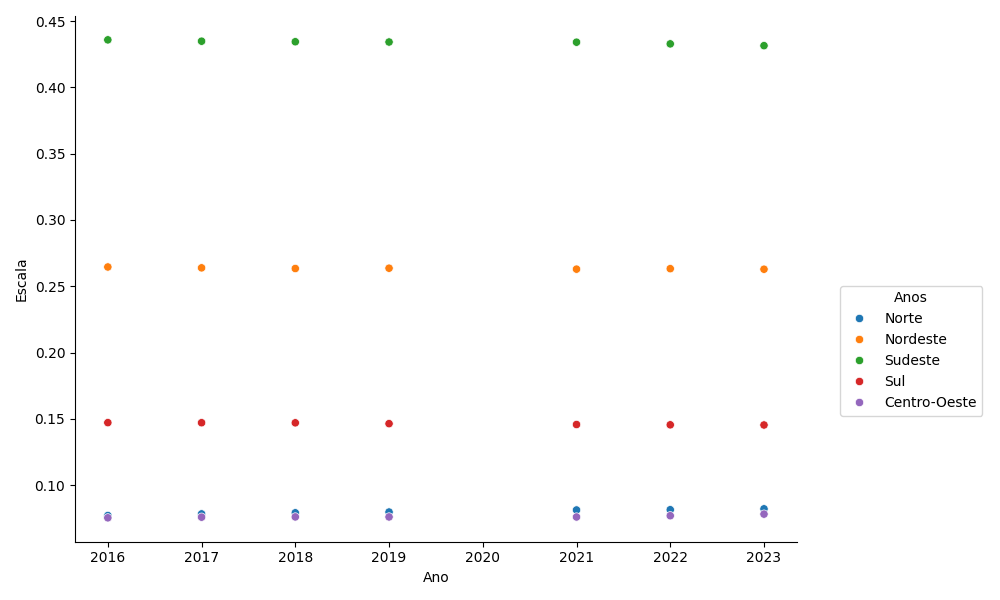
\includegraphics[width=1\linewidth]{figuras/internet/distribuicao_uso_internet_regioes.png}
    \label{fig:distribuicao_uso_internet_regioes}
    \footnotesize{Fonte: \cite{pnda_continua_anual_2016_2023}.}
\end{figure}

Note-se que todas as regiões seguem uma tendência de uso de internet, de modo que mesmo que o número de usuários aumente, uma região não ultrapassará outra. Há 4 classificações, pois as Regiões Centro-Oeste e Região Norte têm uma o índice mais baixo no uso nos anos de 2016-2019 e 2021-2023, estando na 4a classificação. A 3a classificação é ocupada pela Região Sul, seguido da Região Nordeste. A Região Sudeste ocupa a 1a posição.

Para entender a figura \ref{fig:distribuicao_uso_internet_regioes}, fez-se um análise da correlação de Pearson com o índice de uso de internet com a população e densidade populacional de cada região nos anos de 2016-2019 e 2021-2023.